\documentclass[11pt]{beamer}
\usepackage{amsmath}
\usepackage{amsfonts}
\usepackage{amssymb}
\usepackage{graphicx}
\usetheme{CambridgeUS}
\usepackage{xeCJK}
\usepackage{hyperref}
\usepackage{listings}
\usepackage{multirow}

\begin{document}
	\author{宋建勋 \\ 21732100}
	\title[汽油辛烷值定量分析]{基于支持向量机与卷积神经网络的 \\ 汽油辛烷值定量分析}
	%\subtitle{}
	%\logo{}
	%\institute{}
	\date{2017 年 11 月 14 日}
	%\subject{}
	%\setbeamercovered{transparent}
	%\setbeamertemplate{navigation symbols}{}
	\begin{frame}[plain]
		\maketitle
	\end{frame}
	\begin{frame}{摘要}
		这里简要介绍了支持向量机与卷积神经网络的工作原理,然后对实验数据进行了必要的预处理,并使用支持向量回归和卷积神经网络两种方法构建了光谱与辛烷值之间的模型,并对两者的结果进行了评价与分析。
		
		
		\bigskip 其中支持向量机的回归误差复相关系数达到了 $R^2=0.9746$ ,而卷积神经网络则达到了 $R^2=0.9921$,均优于主成分回归等大部分统计学方法。
		作为两种通用的模型,这两者均较好的解决了近红外光谱的分析问题,达到了较为满意的精度。
	\end{frame}
	
	\begin{frame}{目录}
		\tableofcontents
	\end{frame}
	\section{引言}
	\begin{frame}{引言}
		\begin{block}{参数意义}
			汽油在气缸中爆震燃烧时燃烧不完全、震动强烈,容易造成机件受损。
			汽油辛烷值是衡量汽油在气缸内抗爆震燃烧能力的一种指标。
		\end{block}
		
		\begin{block}{检测方法}
			红外光谱法、气相色谱法。
			
			近红外光谱法 (NIR) 由于成本低廉、速度快、无排放物等优点,逐渐成为车用汽油辛烷值测定的主流技术。
		\end{block}
		\begin{block}{目前问题}
			NIR测量结果维数较多,各维度间具有一定程度的相关性,数据的分析处理则较为困难,基本的统计学方法如线性回归、主成分分析等效果一般。
		\end{block}
	\end{frame}
	\begin{frame}{工作环境}
		\noindent 本文使用的软件平台如下:
		\begin{itemize}
			\item openSUSE Tumbleweed + Linux Kernel 4.13.9
			\item Python 3.6 + pip
			\item libsvm
			\item Keras + TensorFlow
		\end{itemize}
	\end{frame}
	
	\begin{frame}
		\begin{block}{openSUSE Tumbleweed + Linux Kernel 4.13.9}
			Linux 是一套具有多用户、多任务、多线程和多CPU支持的开源类 Unix 操作系统。
			由于开源, Linux 还被移植到许多嵌入式系统上。
		\end{block}
		\begin{block}{Python}
			Python 是一种开源的面向对象的解释型编程语言,对科学计算具有良好的支持,拥有诸如 NumPy 、 SciPy 、 MatPlotLib 等诸多开源代码库。
		\end{block}
		\begin{block}{libsvm}
			libsvm是台湾大学林智仁教授等开发设计的一个简单、易于使用和快速有效的SVM模式识别与回归的软件包,基于 BSD 协议开源。
		\end{block}
		\begin{block}{Keras + TensorFlow}
			TensorFlow 由 Google 开发,主要用于机器学习和深度神经网络。
			Keras 则是一个在其上层,为了支持快速的原型实验而生的高层神经网络 API。
		\end{block}
	\end{frame}
	\section{数据预处理}
	\begin{frame}{数据预处理}
		光谱仪所采集的原始光谱图,除了受样品自身的基团组成与含量影响外,还会被样品颜色与杂质、检测器噪声所干扰。
		
		此外,光源强度、探头与样品的矩离、检测器灵敏度等因素也影响着光谱的强度。
		
		因此在对光谱进行建模前,需要通过适当的手段进行预处理,以便消除光谱数据中与样品基团组成无关的信息。	
	\end{frame}
	\begin{frame}{数据预处理}{原始数据}
		\begin{figure}
			\centering
			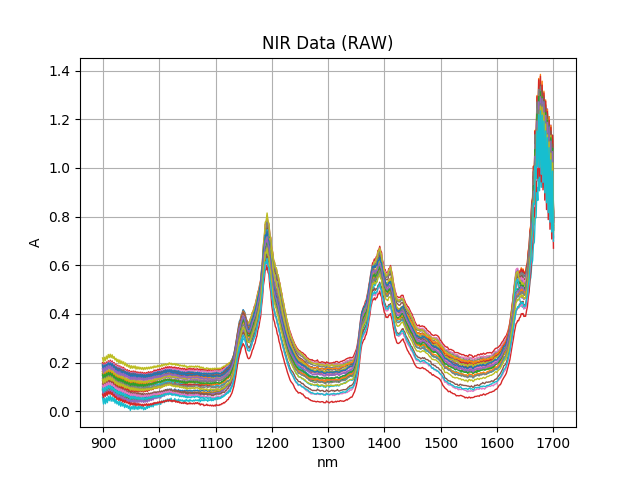
\includegraphics[height=0.7\textheight]{../img/raw}
		\end{figure}
	\end{frame}
	
	\begin{frame}{数据预处理}{多项式卷积平滑}
		\begin{figure}
			\centering
			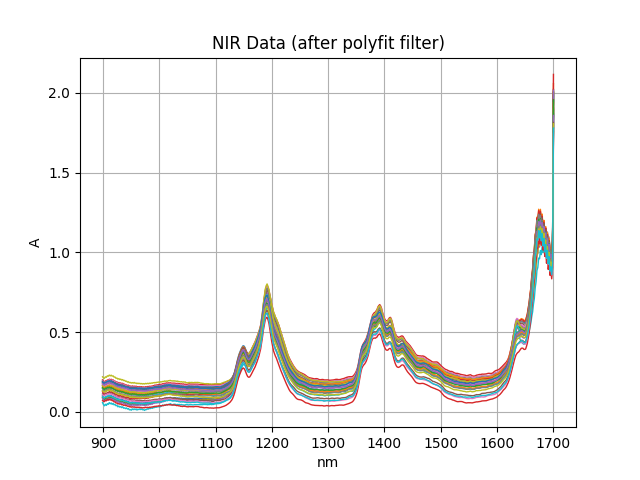
\includegraphics[height=0.7\textheight]{../img/filter}
		\end{figure}
	\end{frame}
			
	\begin{frame}{数据预处理}{基线校正}
		\begin{figure}[h]
			\centering
			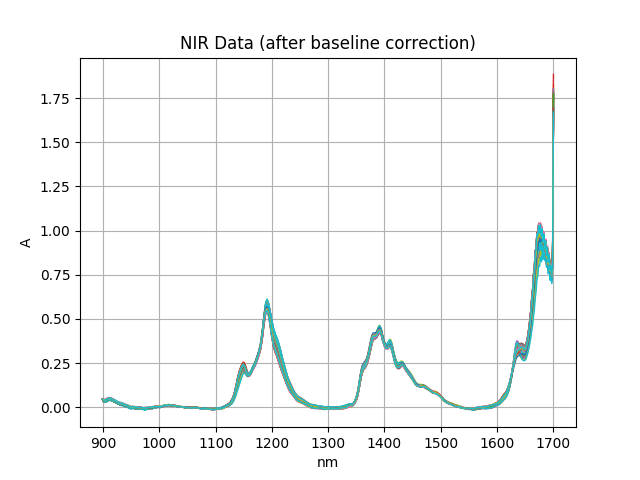
\includegraphics[height=0.7\textheight]{../img/baseline}
		\end{figure}
	\end{frame}
			
	\begin{frame}{数据预处理}{多项式卷积微分}
		\begin{figure}
			\centering
			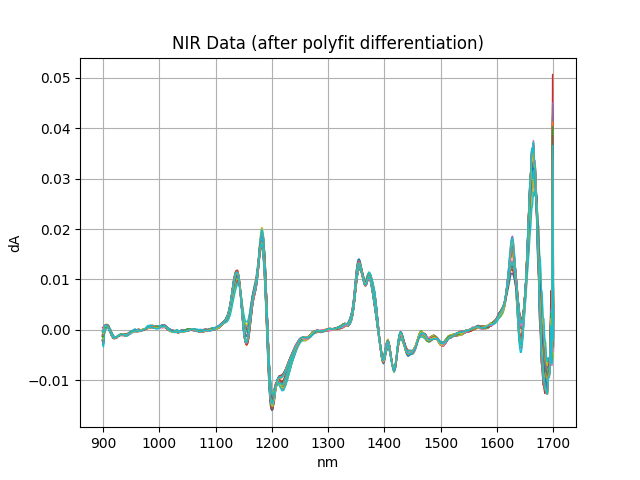
\includegraphics[height=0.7\textheight]{../img/diff}
		\end{figure}
	\end{frame}
	\section{相关性分析}
	\begin{frame}{相关性分析}
		\begin{columns}
			\column{0.3\linewidth}
			相关性分析用于考察光谱信息与待测参数的相关程度。
			
			\bigskip 若光谱各频率与待测参数的相关性均非常低,那么无论使用什么算法,通过分析光谱数据来获得待测参数都会非常困难。
			\column{0.7\linewidth}
			\begin{figure}
				\centering
				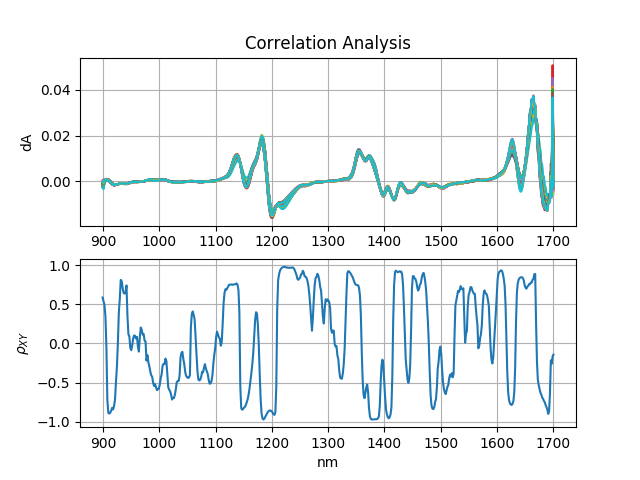
\includegraphics[width=\linewidth]{../img/correlation}
			\end{figure}
		\end{columns}
	\end{frame}
			
	\section{支持向量机}
	\begin{frame}{支持向量机}{理论介绍}
		\begin{block}{适用场景}
			用来解决二分类问题的一种模型,也可以扩展到多分类、回归问题。
		\end{block}
		\begin{block}{基本思想}
			\begin{itemize}
				\item (线性可分)寻找间隔最大的两张平行的超平面,样本点分居两侧;
				\item (近似线性可分)带惩罚地允许样本点越过超平面。
			\end{itemize}
		\end{block}
		\begin{block}{非线性拓展}
			\begin{itemize}
				\item 将线性不可分样本空间映射至高维空间,进而线性可分;
				\item 核函数的优良性质简化了高维空间的计算。
			\end{itemize}
		\end{block}
	\end{frame}
	\begin{frame}{支持向量机}{理论介绍}
		\begin{figure}[h]
			\centering
			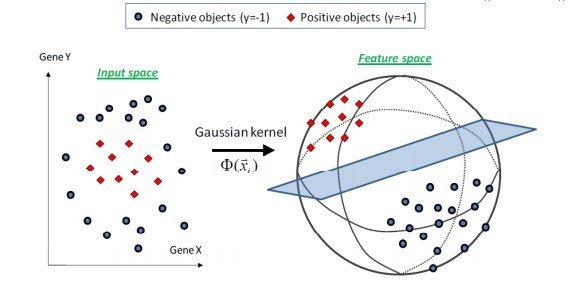
\includegraphics[width=\linewidth]{img/线性不可分到线性可分}
		\end{figure}
	\end{frame}
	\begin{frame}{支持向量机}{理论介绍}
		\begin{columns}
			\column{0.4\linewidth}
			\begin{block}{支持向量回归}
				\begin{itemize}
					\item 人为在高维空间中增加一维,即带测参数的维度;
					\item 寻找间隔最大的超平面,转换为求解距离各点距离和最小的超平面。
				\end{itemize}
			\end{block}
			\column{0.55\linewidth}
			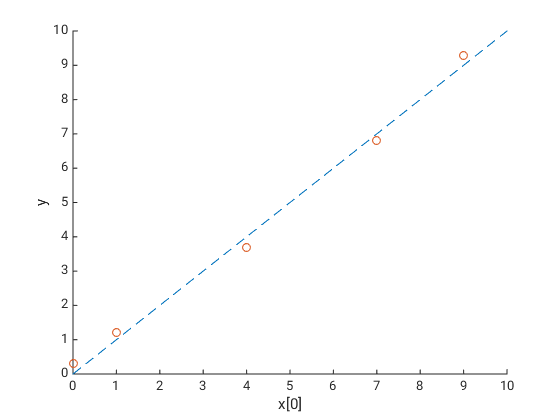
\includegraphics[width=\linewidth]{img/SVR}
		\end{columns}
	\end{frame}
	\begin{frame}{支持向量机}{实现方法}
		这里选用支持向量机的libsvm实现,使用它的的Python接口。该接口主要提供了以下几个函数:
		\begin{itemize}
			\item svm\_train: 用于训练模型,其中参数由字符串的形式传入;
			\item svm\_predict: 用于预测数据,如果给出真值还可以评估模型效果;
			\item svm\_save\_model: 用于保存模型;
			\item svm\_load\_model: 用于加载模型。
		\end{itemize}
	\end{frame}
	\begin{frame}
		其中, svm\_train 能够调整的主要参数有:
		\begin{itemize}\setlength{\itemsep}{0pt}
			\item -s svm\_type : 设置 SVM 类型 (default 0)
			\begin{itemize}
				\item 0 -- C-SVC		(多分类)
				\item 1 -- nu-SVC	(多分类)
				\item 2 -- 一分类 SVM
				\item 3 -- epsilon-SVR	(回归)
				\item 4 -- nu-SVR		(回归)
			\end{itemize}
			\item -t kernel\_type : 设置核函数类型 (default 2)
			\begin{itemize}
				\item 0 -- 线性: $u'*v$
				\item 1 -- 多项式: $(\gamma * u' * v + coef_0)^{degree}$
				\item 2 -- 径向基函数: $e^{-\gamma * \left|u-v\right|^2}$
				\item 3 -- sigmoid 函数: $\tanh(\gamma * u' * v+coef_0)$
			\end{itemize}
			\item -c cost : 设置 C-SVC、 epsilon-SVR 和 nu-SVR 的惩罚系数 (default 1)
		\end{itemize}
	\end{frame}
	\begin{frame}{支持向量机}{训练与结果}
		\begin{block}{步骤}
			\begin{enumerate}
				\item 对各维度进行标准化;
				\item 再要求组织输入数据;
				\item 2:1 划分训练集与测试集;
				\item 选择核函数与参数,训练,交叉检验。
			\end{enumerate}
		\end{block}
		\begin{block}{支持向量机}{核函数比较}
			\scalebox{0.87}{
			\begin{tabular}{r|c|c|c|c|c|c|c|c}
				\hline
				\footnotesize 核函数&\footnotesize 线性&\footnotesize 多项式&\footnotesize 径向基&\multicolumn{5}{c}{Sigmoid} \\
				\hline
				\footnotesize 惩罚系数&\multicolumn{4}{c|}{$c = 1$}&0.8&1.2&1.6&2\\
				\hline
				SEC&0.6540&1.1182&0.8978&0.5905&0.6306&0.5104&0.4835&0.6488\\
				$R^2$&0.9536&0.8643&0.9126&0.9622&0.9569&0.9717&0.9746&0.9543\\
				\hline
			\end{tabular}
			}
		\end{block}
	\end{frame}
	\begin{frame}
		\begin{minipage}{\linewidth}
			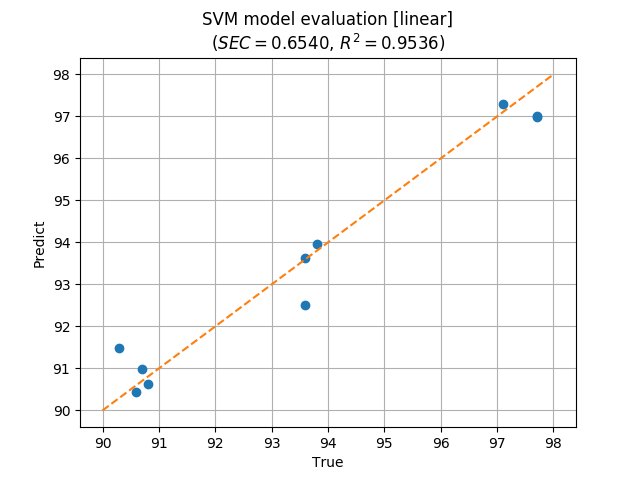
\includegraphics[width=0.5\linewidth]{../img/svm_result_t0}
			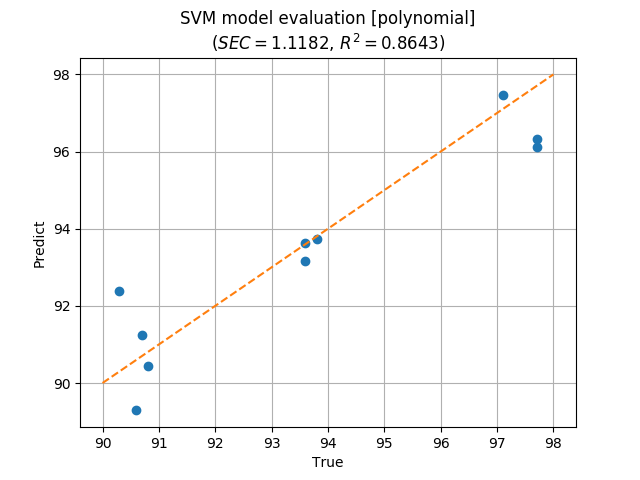
\includegraphics[width=0.5\linewidth]{../img/svm_result_t1} \\
			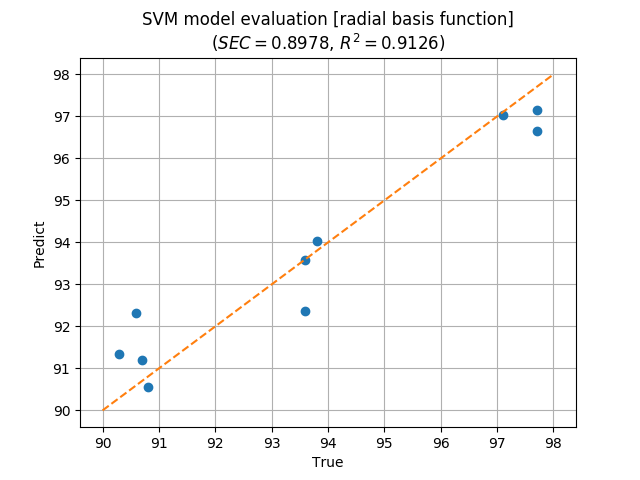
\includegraphics[width=0.5\linewidth]{../img/svm_result_t2}
			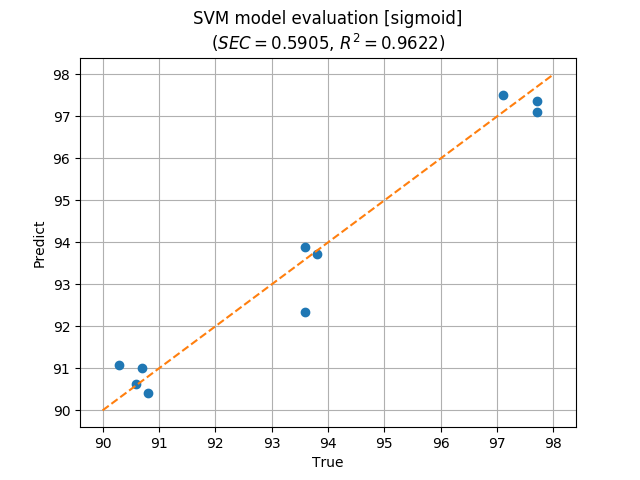
\includegraphics[width=0.5\linewidth]{../img/svm_result_t3}
		\end{minipage}
	\end{frame}
	\begin{frame}
		\begin{minipage}{\linewidth}
			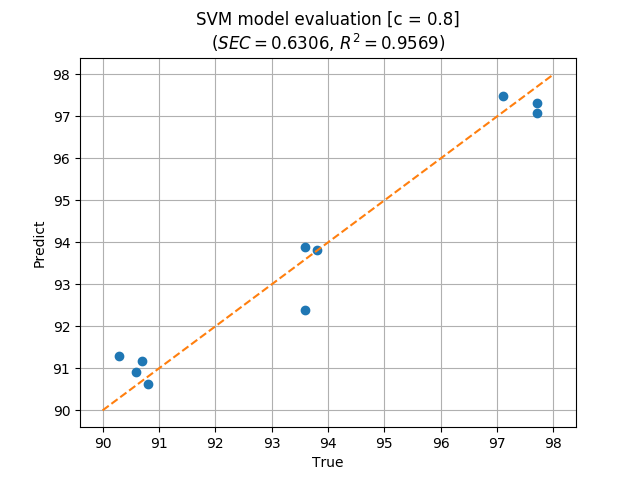
\includegraphics[width=0.5\linewidth]{../img/svm_result_t3_c0_8}
			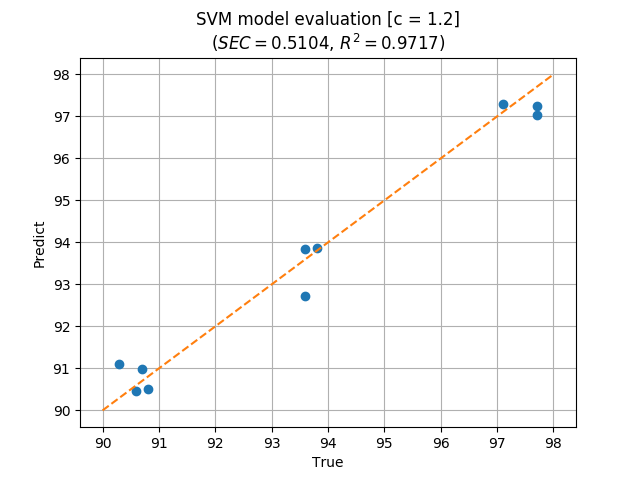
\includegraphics[width=0.5\linewidth]{../img/svm_result_t3_c1_2} \\
			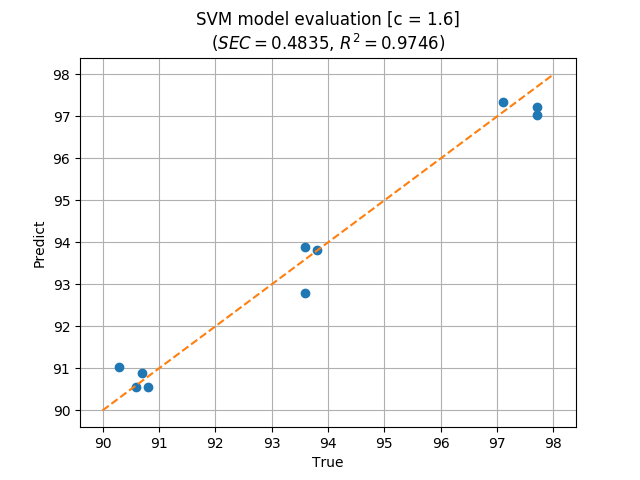
\includegraphics[width=0.5\linewidth]{../img/svm_result_t3_c1_6}
			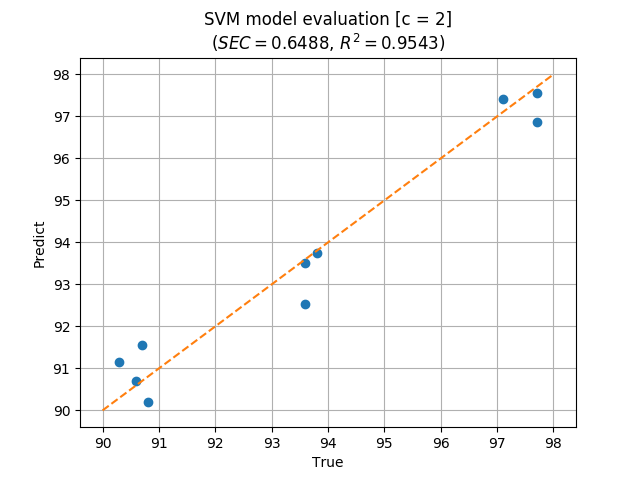
\includegraphics[width=0.5\linewidth]{../img/svm_result_t3_c2}
		\end{minipage}
	\end{frame}			
	\section{卷积神经网络}
	\begin{frame}{卷积神经网络 (Convolutional Neural Network, CNN)}
		\begin{block}{特点}
			\begin{itemize}
				\item CNN 是一种前馈神经网络,常用于处理图像数据。
				\item 图像数据相邻像素点间具有关联性;
				\item 使用卷积层和池化层,用于提取相邻像素点间的关联;
				\item 相比于全连接层,网络的总参数量降低。
			\end{itemize}
		\end{block}
		\begin{block}{适用性}
			在光谱数据处理中,由于样品在相邻波长的响应也具有关联性,因此 CNN 也应当适用于光谱分析。
		\end{block}
	\end{frame}
	\begin{frame}{卷积神经网络 (Convolutional Neural Network, CNN)}{网络结构}
		\begin{block}{为什么需要好的网络结构?}
			\begin{minipage}{0.55\linewidth}
				\begin{itemize}
					\item 参数太少可能会抓不到特征
					\item 参数太多训练很慢;
					\item 参数太多可能会振荡,无法收敛;
					\item 可能落入全局最优解。
				\end{itemize}
			\end{minipage}
			$\Longrightarrow$ 
			\begin{minipage}{0.3\linewidth}
				安排合理的网络结构 \\ 减少无用参数
			\end{minipage}
		\end{block}
		\begin{block}{LeNet-5}
			\centering
			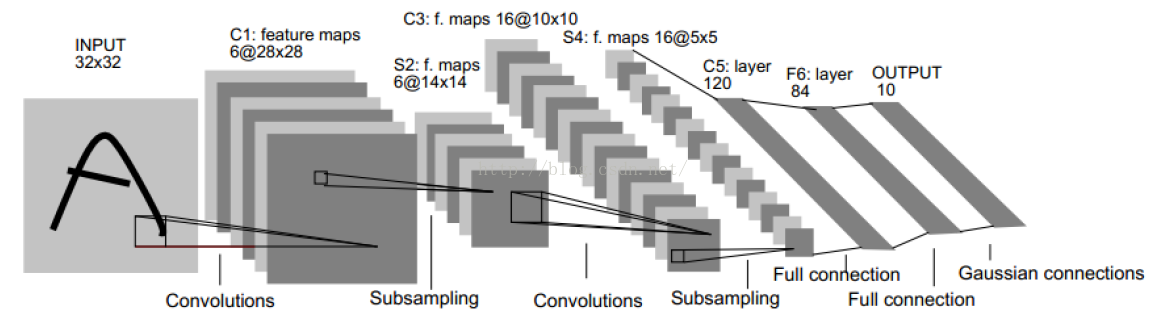
\includegraphics[width=0.8\linewidth]{img/LeNet-5}
		\end{block}
	\end{frame}
	\begin{frame}{卷积神经网络 (Convolutional Neural Network, CNN)}{网络结构}
		\begin{itemize}
			\item 参考了 LeNet 的网络结构;
			\item 先进行了4次卷积+池化操作,再经过全连接层到达输出层。
			\item 激活函数: ReLu;
			\item 损失函数: MSE;
			\item 优化器: Adam 。
			\item 为了防止模型过拟合,当精度经过连续数轮训练没有改善时,还要及时提前停止训练。
		\end{itemize}
	\end{frame}
	\begin{frame}{卷积神经网络 (Convolutional Neural Network, CNN)}{网络结构}
		\centering
		\scalebox{0.7}{\lstinputlisting[basicstyle=\fontsize{8.8pt}{9.8pt}\selectfont]{../cnn-model.txt}}
	\end{frame}
	\begin{frame}{卷积神经网络 (Convolutional Neural Network, CNN)}{训练与结果}
		\begin{block}{步骤}
			\begin{enumerate}
				\item 对每条光谱数据进行标准化;
				\item 按照 TensorFlow 的格式,组织输入数据;
				\item 按 $2:1$ 划分为训练集和测试集;
				\item 训练模型并检测结果。
			\end{enumerate}
		\end{block}
		\begin{block}{训练结果}
			\begin{itemize}
				\item 训练速度慢于 SVR ;
				\item 训练结果具有随机性,每次训练结果均不一样;
				\item 回归标准误差 $SEC = 0.2694$,回归误差复相关系数 $R^2 = 0.9921$ ;
				\item 优于 PCA 和 SVR ,与 4 主元 PLS 效果相近。
			\end{itemize}
		\end{block}
	\end{frame}

	\begin{frame}
		\centering
		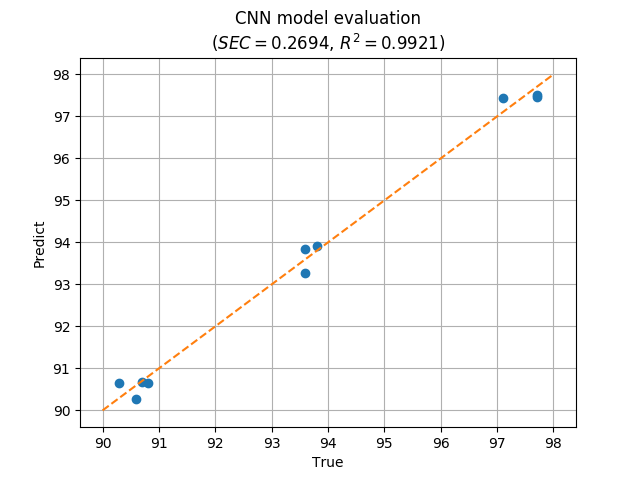
\includegraphics[width=\linewidth]{../img/cnn_result}
	\end{frame}
	\begin{frame}
		\begin{block}{CNN 的预测效果好于 SVR,为什么?}
			\bigskip
			\begin{itemize}
				\item 一般来说,神经网络需要比支持向量回归更多的训练数据;
				\item CNN 的卷积层相比于全连接层,能够更加有效的提取光谱的特征;
				\item 相比于 SVM,CNN 的可塑性也更好。
			\end{itemize}
		\end{block}
	\end{frame}
	\section{总结}
	\begin{frame}{总结}
		\begin{block}{各模型预测效果}
			\scalebox{0.73}{
				\begin{tabular}{r|c|c|c|c|c|c|c|c||c|c}
					\hline
					\multicolumn{9}{c||}{SVR} & \multicolumn{1}{c|}{\multirow{3}{*}{CNN}}\\
					\cline{1-9}
					\footnotesize 核函数&\footnotesize 线性&\footnotesize 多项式&\footnotesize 径向基&\multicolumn{5}{c||}{Sigmoid}& \\
					\cline{1-9}
					\footnotesize 惩罚系数&\multicolumn{4}{c|}{$c = 1$}&0.8&1.2&1.6&2&\\
					\hline
					SEC&0.6540&1.1182&0.8978&0.5905&0.6306&0.5104&0.4835&0.6488&0.2694&SEC\\
					$R^2$&0.9536&0.8643&0.9126&0.9622&0.9569&0.9717&0.9746&0.9543&0.9921&$R^2$\\
					\hline
				\end{tabular}
			}
		\end{block}
		\begin{block}{问题}
			\begin{itemize}
				\item 数据样本太少,机器学习一般需要大量样本,30条一般来说不够;
				\item 误差追溯困难,内部机理复杂,难以理解;
			\end{itemize}
		\end{block}
		\begin{block}{优势}
			\begin{itemize}
				\item 两种方法准确度高于一般统计方法,CNN 与 4 主元 PLS 效果相当;
				\item 更换分析仪器或油品产地后,只需要追加新的数据即可恢复精度。
			\end{itemize}
		\end{block}
	\end{frame}
	\section{参考资料}
	\begin{frame}{参考资料}
			\begin{thebibliography}{9}
			\bibitem{} 在线分析技术及仪器 - 课程讲义
			\bibitem{} 邓乃扬, 田英杰. 支持向量机:理论、算法与拓展[M]. 科学出版社, 2009.
			\bibitem{} July, pluskid. 支持向量机通俗导论(理解SVM的三层境界)[EB/OL]. [2017-11-05]. \url{http://blog.csdn.net/macyang/article/details/38782399/}.
			\bibitem{} \href{https://github.com/fchollet}{fchollet}. Keras Documentation[EB/OL]. [2017-11-05]. \url{https://keras.io/}.
		\end{thebibliography}
	\end{frame}
	\frame[plain]{\centering FIN. \\ 谢谢观看}
\end{document}